\documentclass{article}
\usepackage{clrscode4e}
\usepackage{tikz}
\usetikzlibrary{fit,positioning}
\usepackage{textcomp}
\usepackage{amsmath}
\usepackage{amssymb}
\usepackage{verbatim}

\begin{document}

\section{Overview}
This document describes one method of learning to plan via program induction.
It uses a simpler version of the generative model described in the other planner document.

A \emph{plan} is a sequence of programs $e_1, e_2, ...$ that are composed to produce $e_1\circ e_2 \circ ...$ and applied to an initial empty plan (an empty list, the identity function, a constant function, etc, depending on the specific domain).
Our domain has a large number of planning tasks.
We wish to learn a grammar such that, when programs are sampled from this grammar and composed to produce plans, they have a high probability of solving one of the planning tasks.
We'll do this using either Monte Carlo EM or AIP.
This document will describe the generative model and detail one means of performing posterior inference.

\section{Generative Model}
We're given $N$ tasks.
For each task $t$ a plan $\rho$ and a plan length $|\rho|$ is sampled, with the length of the plan chosen uniformly from $\{1,2,...,\ell\}$.
There is some problem-dependent $P(t | \rho)\in[0,1]$ which should be higher for plans that do a better job of solving the task, and zero for plans that don't solve the task.

The grammar produces plan $\rho = e_1\circ e_2\circ \cdots \circ e_k$ with probability
$$
P\left( e_1\circ e_2\circ \cdots \circ e_k | G \right) =
\begin{cases}
    \frac{1}{\ell}\prod_i P(e_i | G),& \text{if } 0<k\leq \ell\\
    0,              & \text{otherwise}
\end{cases}
$$
The generative model is illustrated in Fig. 1.

\begin{figure}
\centering
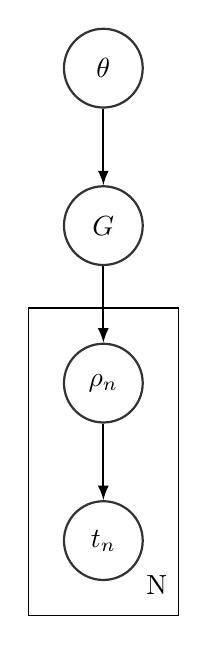
\begin{tikzpicture}
\tikzstyle{main}=[circle, minimum size = 10mm, thick, draw =black!80, node distance = 16mm]
\tikzstyle{connect}=[-latex, thick]
\tikzstyle{box}=[rectangle, draw=black!100]

\node[main, fill = white!100] at (0,2) (lambda)  {$\theta$ };
\node[main, fill = white!100] at (0, 0) (grammar)  {$G$ };
\node[main, fill = white!100] at (0,-2) (psubk) {$\rho_n$ };
\node[main, fill = white!100] at (0,-4) (tsubk) {$t_n$ };
\path (lambda) edge [connect] (grammar);
\path (grammar) edge [connect] (psubk);
\path (psubk) edge [connect] (tsubk);
\node[rectangle, inner sep=0mm, fit= (psubk) (tsubk),label=below right:N, xshift=-1mm, yshift=-8mm] {};
\node[rectangle, inner sep=4.4mm,draw=black!100, fit= (psubk) (tsubk)] {};
\end{tikzpicture}
\caption{Generative model used for the planner}
\end{figure}

\section{Inference}
Following the Monte Carlo EM derivation described in the ``inference'' document, we want to find the grammar maximizing
$$
\log P(G|\theta)+\sum_n \mathbb{E}_{q_n}\left[ \log P(\rho_n | G) \right]
$$
where
$$
\tilde{q}_n(e_1\cdots e_k) = P(t_n | e_1\cdots e_k)\prod_i P(e_i | G)
$$
Now, if we can sample from $\tilde{q}$, we're done.
We could just sample/enumerate random plans from $G$ and then do likelihood weighting, but if our frontier is of order $10^4$ or so, this will quickly become impractical for $\ell$ of order $10^1$.
Instead, we'll use MCMC to get samples from a proposal distribution, which we'll then reweight.
\subsection{Planning via MCMC}
We'll draw samples (plans) from a distribution $\tilde{g}(\cdot)$ that will serve as a proposal distribution for the expectation w.r.t. $q_n$.
This MCMC algorithm is not Metropolis-Hastings, but it has a stationary distribution which is similar to $q_n$.
Given a plan $\rho$ with $|\rho|<\ell$, the proposal distribution $h(\cdot | \cdot)$ is
$$
h(\rho e | \rho) \propto P(t|\rho e) P(e|G)
$$
A plan $|\rho|=\ell$ has $h(\emptyset | \rho)=1$.
Intuitively, the sampler is growing out a plan, starting from $\emptyset$, sampling the next move according to the posterior distribution upon the next program (greedy one-step lookahead).
The stationary distribution of this Markov chain is
$$
\tilde{g} (e_1 e_2 \cdots e_k) = P(e_1 | G) P(e_2 | G) \cdots P(e_k | G) P(t | e_1) P(t | e_1e_2) \cdots P(t | e_1e_2\cdots e_k)
$$
as can be verified by observing that $\tilde{g}(\rho e)=h(\rho e | \rho) \tilde{g}(\rho)$.
So, we reweight a plan $\rho=e_1e_2\cdots e_k$ by the quantity
$$
\frac{\tilde{q}}{\tilde{g}} = \frac{1}{P(t|e_1)P(t|e_1e_2)\cdots P(t|e_1e_2\cdots e_{k-1})}
$$
Each plan of length $\ell$ sampled contributes $\ell$ total samples (all prefixes of the plan).
Each total plan $\rho=e_1\cdots e_\ell$ contributes the following quantity to the maximization problem in $G$ (up to a normalizing constant):
\begin{eqnarray*}
&&\sum_{k\leq\ell} \frac{\tilde{q}(e_1\cdots e_k)}{\tilde{g}(e_1\cdots e_k)} \sum_{j\leq k} \log P(e_j | G)\\
&=&\sum_{k\leq\ell} \frac{1}{P(t|e_1)P(t|e_1e_2)\cdots P(t|e_1e_2\cdots e_{k-1})} \sum_{j\leq k} \log P(e_j | G)\\
&=&\sum_{j\leq \ell} w_j\log P(e_j | G)
\end{eqnarray*}
where I've introduced the quantities
$$
w_j=\sum_{m\geq j} \frac{1}{P(t|e_1)P(t|e_1e_2)\cdots P(t|e_1\cdots e_{j-1})}
$$
The $w_j$'s factor in a nice way that allows them to be computed in linear time using a dynamic program.
\footnote{The sums for $w_j$ end up being the partition function if $j=1$ and is a sort of ``truncated partition function'' for $j>1$.
For the $j>1$ case, the weights $w_j$ are what the partition function \emph{would have been} if the plan had started with programs $e_{k<j}$ for free.}
The following procedure samples a plan and returns the weights upon each program in that plan, along with the partition function:
\begin{codebox}
\Procname{$\proc{MCMC-Plan}(\rho, \mbox{\id{reciprocalLikelihoods}})$}
\li \Comment{Draw the next program in the plan}
\li \id{e} $\sim$ $P(\rho\cdot | t, G)$
\li \Comment{If the plan should be extended, recurse, creating the suffix of the plan}
\li \If $|\rho e|<\ell$ \Then
\li \id{suffixZ}, \id{suffixWeights} = \func{MCMC-Plan}$(\rho e, \mbox{\id{reciprocalLikelihoods}}/P(t|\rho e))$
\li \Else
\li \id{suffixZ}, \id{suffixWeights} = $0$, $\emptyset$
\li \End
\li \id{Z} = \id{suffixZ} + \id{reciprocalLikelihoods}
\li \Return \id{Z}, $\{(e, \mbox{\id{Z}})\}\cup \mbox{\id{suffixWeights}}$
\end{codebox}
where \emph{reciprocalLikelihoods} is set to $1$ initially.

It may seem strange that, in the generative model, we produce plans by doing a random walk without any bias towards the target.
However, this is actually to be expected, because the target has not yet been generated.
When performing inference, we condition upon the random walk hitting the target; this conditioning has the same role as planning would have.
Rather than use rejection sampling, we use a stochastic, greedy search (the MCMC procedure) to bias us towards plans that hit the targets.
The $w_j$'s serve to correct for the biases introduced by this stochastic search.
They may also be thought of as ``rewards'' for each program used in a plan.
Note that their dependence upon likelihood at each point in the plan is non-trivial; initial programs get some of the credit for subsequent increases in likelihood, as is intuitively correct.

The likelihood isn't the only heuristic that could be used in the stochastic greedy search.
If we had some other heuristic, $\hat{\mbox{H}}$, one reasonable proposal for the MCMC walk would be the Boltzman distribution:
$$
h(\rho e | \rho) \propto \exp\left(-\hat{\mbox{H}}(\rho e) + \log P(e|G)\right)
$$

\end{document}
